\pagebreak
\section{Simulation Analysis}
\label{sec:simulation}

\subsection{Operating Point Analysis for t<0}

Table~\ref{tab:passo1} shows the simulated operating point results for the RC circuit
for t<0. 

\begin{table}[h]
  \centering
  \begin{tabular}{|l|r|}
    \hline    
    {\bf Name} & {\bf Value [V or A]} \\ \hline
    \input{../sim/passo1}
  \end{tabular}
  \caption{Operating point for RC circuit for t<0. A variable preceded by @ is of type {\em current}
    and expressed in Ampere; other variables are of type {\it voltage} and expressed in
    Volt.}
  \label{tab:passo1}
\end{table}

The relative error between the theoretical and simulation values is of the order of magnitude of 10 to the power of -5 \%. The errors are insignificant due to the simplicity of the circuit.

\subsection{Determining initial conditions}

To be able to plot the voltages for t>0, we need to obtain the initial conditions of the capacitor nodes.

Table~\ref{tab:passo2} shows the simulated operating point results for the same circuit with its independent source turned off and with the capacitor replaced with a voltage source $V_x$, whose value is $V_6$-$V_8$, $V_6$ and $V_8$ being the nodal voltages obtained in the previous section. 

\begin{table}[h]
  \centering
  \begin{tabular}{|l|r|}
    \hline    
    {\bf Name} & {\bf Value [V or A]} \\ \hline
    \input{../sim/passo2}
  \end{tabular}
  \caption{Operating point results for the circuit described in this section. A variable preceded by @ is of type {\em current}
    and expressed in Ampere; other variables are of type {\it voltage} and expressed in
    Volt.}
  \label{tab:passo2}
\end{table}

The relative error between the theoretical and simulation values is of the order of magnitude of 10 to the power of -5 \%. The errors are insignificant due to the simplicity of the circuit.

\subsection{Natural Solution}

Figure~\ref{fig:natsol} shows the simulated transient analysis results for natural solution of $V_6(t)$. The initial solutions of $V_6$ and $V_8$ were provided by the octave script to simplify the project, since the relative error is irrelevant. 

\begin{figure}[h] \centering
\includegraphics[width=0.3\linewidth]{../sim/tnr.pdf}
\caption{Natural Solution of $V_6(t)$ for t>=0.}
\label{fig:natsol}
\end{figure}

Compared to the theoretical analysis results, one
notices that the plots of figure \ref{fig:solnat} and figure \ref{fig:natsol} are very similar and any differences can be explained by aproximation errors.

\subsection{Total solution}

Figure~\ref{fig:totalsolV6} shows the simulated transient analysis results for $V_6(t)$.

\begin{figure}[h] \centering
\includegraphics[width=0.3\linewidth]{../sim/trv6.pdf}
\caption{Total solution of $V_6(t)$.}
\label{fig:totalsolV6}
\end{figure}

Figure~\ref{fig:totalsolVs} shows the simulated transient analysis results for $V_s(t)$.

\begin{figure}[h] \centering
\includegraphics[width=0.3\linewidth]{../sim/trvs.pdf}
\caption{Total solution of $V_s(t)$.}
\label{fig:totalsolVs}
\end{figure}

Compared to the theoretical analysis results, one
notices that, for t>0, the plots of figure \ref{fig:soltotal} and figures \ref{fig:totalsolV6} and \ref{fig:totalsolVs} are very similar and any differences can be explained by aproximation errors.

\subsection{Frequency Response}

Figure~\ref{fig:acm} shows the magnitude response for $V_6(t)$ and $V_s(t)$. 

\begin{figure}[h] \centering
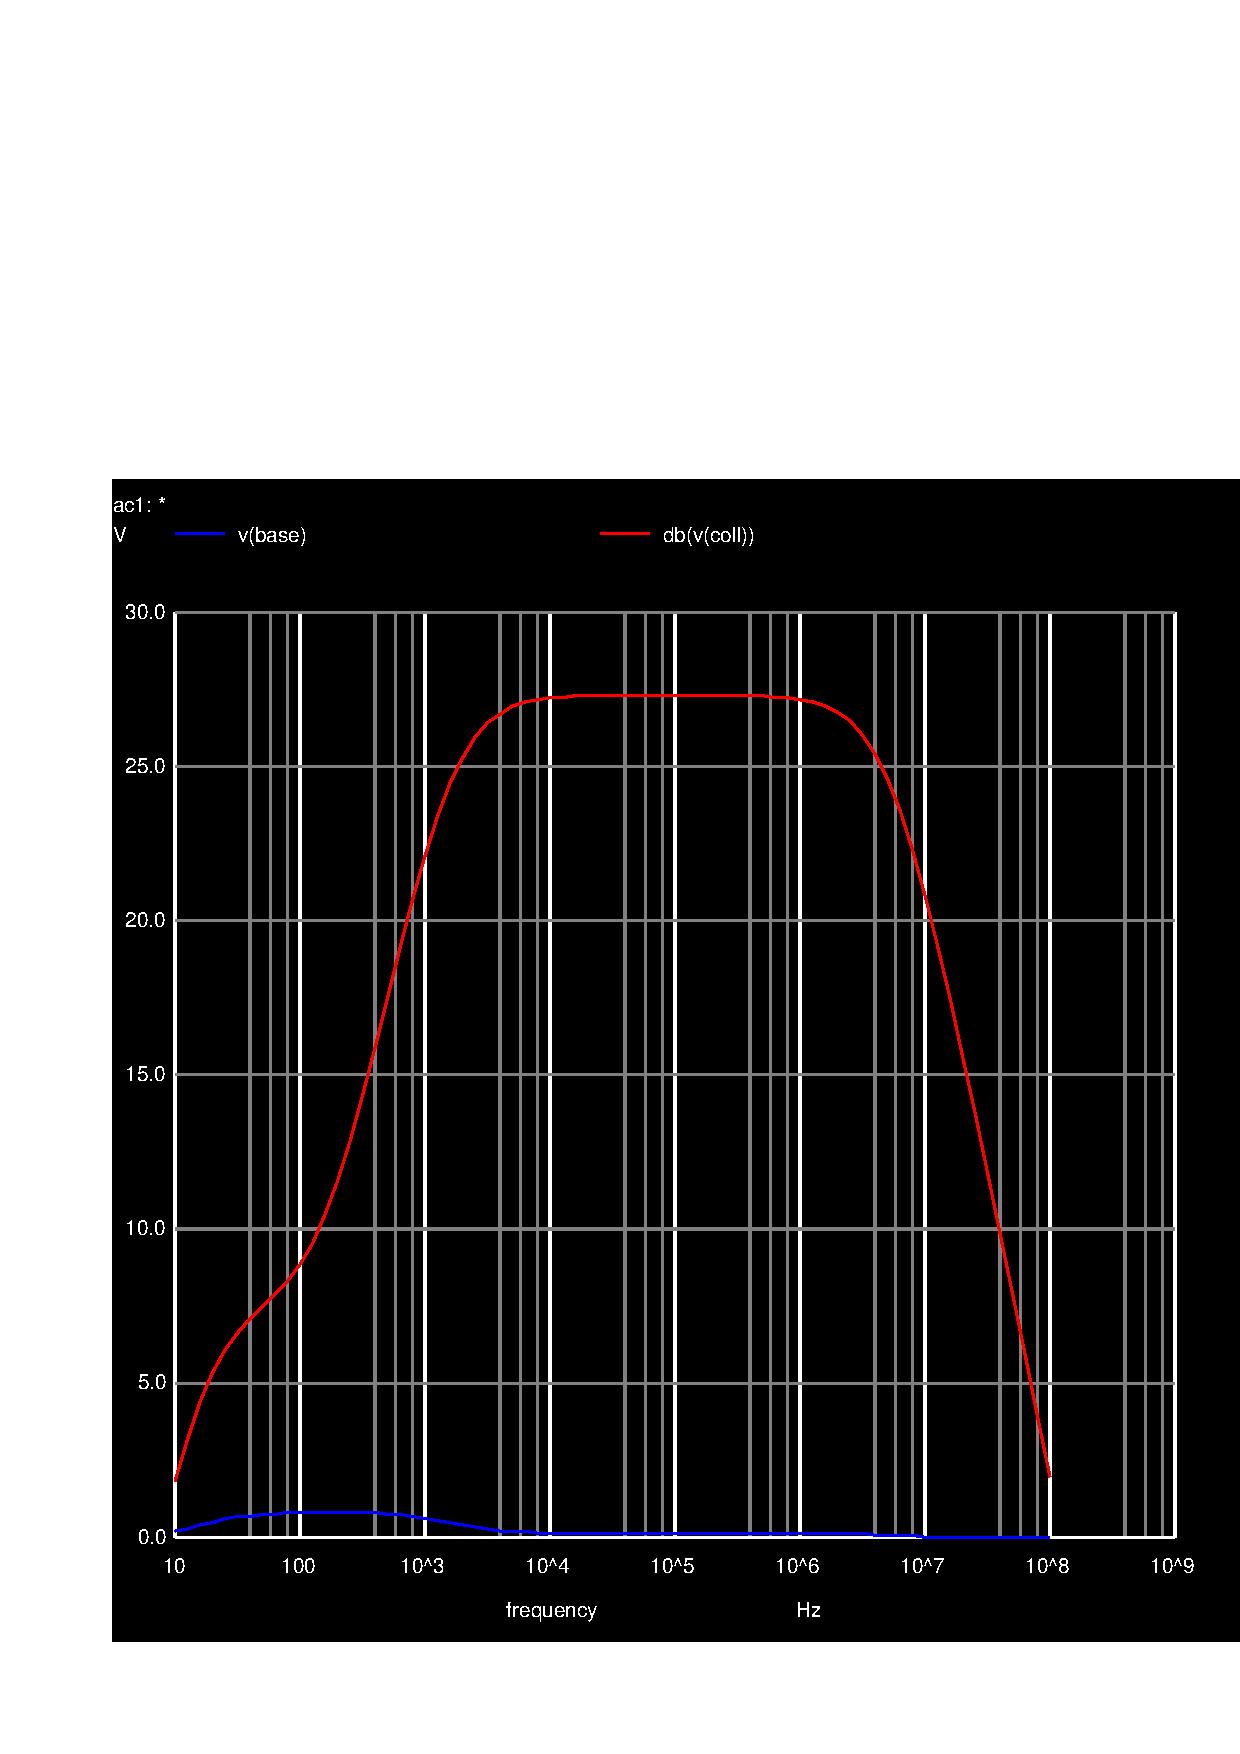
\includegraphics[width=0.6\linewidth]{../sim/acm.pdf}
\caption{Magnitude Response of $V_6(t)$ (blue) and $V_s(t)$ (red).}
\label{fig:acm}
\end{figure}

Compared to the theoretical analysis results of figure \ref{fig:mag}, we can see that the simulated results in figure \ref{fig:acm} are very similar and any differences can be explained by aproximation errors.

The magnitude of $V_s(t)$ doesn't change with the frequency of the signal and therefore it always´1 (0 in dB). However, the magnitude of $V_6$ changes with the frequency, firstly reducing and then staying constant.

Figure \ref{fig:acm} shows the phase response for $V_6(t)$ and $V_s(t)$.

\begin{figure}[h] \centering
\includegraphics[width=0.6\linewidth]{../sim/pr.pdf}
\caption{Phase Response of $V_6(t)$ (blue) and $V_s(t)$ (red).}
\label{fig:pr}
\end{figure}

Compared to the theoretical analysis results of figure \ref{fig:phase}, one notices that the simulated results in figure \ref{fig:pr} are very similar and any differences can be explained by aproximation errors.

